% Options for packages loaded elsewhere
\PassOptionsToPackage{unicode}{hyperref}
\PassOptionsToPackage{hyphens}{url}
\PassOptionsToPackage{dvipsnames,svgnames,x11names}{xcolor}
%
\documentclass[
  11pt,
]{article}

\usepackage{amsmath,amssymb}
\usepackage{iftex}
\ifPDFTeX
  \usepackage[T1]{fontenc}
  \usepackage[utf8]{inputenc}
  \usepackage{textcomp} % provide euro and other symbols
\else % if luatex or xetex
  \usepackage{unicode-math}
  \defaultfontfeatures{Scale=MatchLowercase}
  \defaultfontfeatures[\rmfamily]{Ligatures=TeX,Scale=1}
\fi
\usepackage{lmodern}
\ifPDFTeX\else  
    % xetex/luatex font selection
\fi
% Use upquote if available, for straight quotes in verbatim environments
\IfFileExists{upquote.sty}{\usepackage{upquote}}{}
\IfFileExists{microtype.sty}{% use microtype if available
  \usepackage[]{microtype}
  \UseMicrotypeSet[protrusion]{basicmath} % disable protrusion for tt fonts
}{}
\makeatletter
\@ifundefined{KOMAClassName}{% if non-KOMA class
  \IfFileExists{parskip.sty}{%
    \usepackage{parskip}
  }{% else
    \setlength{\parindent}{0pt}
    \setlength{\parskip}{6pt plus 2pt minus 1pt}}
}{% if KOMA class
  \KOMAoptions{parskip=half}}
\makeatother
\usepackage{xcolor}
\usepackage[margin=1in]{geometry}
\setlength{\emergencystretch}{3em} % prevent overfull lines
\setcounter{secnumdepth}{-\maxdimen} % remove section numbering
% Make \paragraph and \subparagraph free-standing
\makeatletter
\ifx\paragraph\undefined\else
  \let\oldparagraph\paragraph
  \renewcommand{\paragraph}{
    \@ifstar
      \xxxParagraphStar
      \xxxParagraphNoStar
  }
  \newcommand{\xxxParagraphStar}[1]{\oldparagraph*{#1}\mbox{}}
  \newcommand{\xxxParagraphNoStar}[1]{\oldparagraph{#1}\mbox{}}
\fi
\ifx\subparagraph\undefined\else
  \let\oldsubparagraph\subparagraph
  \renewcommand{\subparagraph}{
    \@ifstar
      \xxxSubParagraphStar
      \xxxSubParagraphNoStar
  }
  \newcommand{\xxxSubParagraphStar}[1]{\oldsubparagraph*{#1}\mbox{}}
  \newcommand{\xxxSubParagraphNoStar}[1]{\oldsubparagraph{#1}\mbox{}}
\fi
\makeatother


\providecommand{\tightlist}{%
  \setlength{\itemsep}{0pt}\setlength{\parskip}{0pt}}\usepackage{longtable,booktabs,array}
\usepackage{calc} % for calculating minipage widths
% Correct order of tables after \paragraph or \subparagraph
\usepackage{etoolbox}
\makeatletter
\patchcmd\longtable{\par}{\if@noskipsec\mbox{}\fi\par}{}{}
\makeatother
% Allow footnotes in longtable head/foot
\IfFileExists{footnotehyper.sty}{\usepackage{footnotehyper}}{\usepackage{footnote}}
\makesavenoteenv{longtable}
\usepackage{graphicx}
\makeatletter
\def\maxwidth{\ifdim\Gin@nat@width>\linewidth\linewidth\else\Gin@nat@width\fi}
\def\maxheight{\ifdim\Gin@nat@height>\textheight\textheight\else\Gin@nat@height\fi}
\makeatother
% Scale images if necessary, so that they will not overflow the page
% margins by default, and it is still possible to overwrite the defaults
% using explicit options in \includegraphics[width, height, ...]{}
\setkeys{Gin}{width=\maxwidth,height=\maxheight,keepaspectratio}
% Set default figure placement to htbp
\makeatletter
\def\fps@figure{htbp}
\makeatother
% definitions for citeproc citations
\NewDocumentCommand\citeproctext{}{}
\NewDocumentCommand\citeproc{mm}{%
  \begingroup\def\citeproctext{#2}\cite{#1}\endgroup}
\makeatletter
 % allow citations to break across lines
 \let\@cite@ofmt\@firstofone
 % avoid brackets around text for \cite:
 \def\@biblabel#1{}
 \def\@cite#1#2{{#1\if@tempswa , #2\fi}}
\makeatother
\newlength{\cslhangindent}
\setlength{\cslhangindent}{1.5em}
\newlength{\csllabelwidth}
\setlength{\csllabelwidth}{3em}
\newenvironment{CSLReferences}[2] % #1 hanging-indent, #2 entry-spacing
 {\begin{list}{}{%
  \setlength{\itemindent}{0pt}
  \setlength{\leftmargin}{0pt}
  \setlength{\parsep}{0pt}
  % turn on hanging indent if param 1 is 1
  \ifodd #1
   \setlength{\leftmargin}{\cslhangindent}
   \setlength{\itemindent}{-1\cslhangindent}
  \fi
  % set entry spacing
  \setlength{\itemsep}{#2\baselineskip}}}
 {\end{list}}
\usepackage{calc}
\newcommand{\CSLBlock}[1]{\hfill\break\parbox[t]{\linewidth}{\strut\ignorespaces#1\strut}}
\newcommand{\CSLLeftMargin}[1]{\parbox[t]{\csllabelwidth}{\strut#1\strut}}
\newcommand{\CSLRightInline}[1]{\parbox[t]{\linewidth - \csllabelwidth}{\strut#1\strut}}
\newcommand{\CSLIndent}[1]{\hspace{\cslhangindent}#1}

\makeatletter
\@ifpackageloaded{caption}{}{\usepackage{caption}}
\AtBeginDocument{%
\ifdefined\contentsname
  \renewcommand*\contentsname{Table of contents}
\else
  \newcommand\contentsname{Table of contents}
\fi
\ifdefined\listfigurename
  \renewcommand*\listfigurename{List of Figures}
\else
  \newcommand\listfigurename{List of Figures}
\fi
\ifdefined\listtablename
  \renewcommand*\listtablename{List of Tables}
\else
  \newcommand\listtablename{List of Tables}
\fi
\ifdefined\figurename
  \renewcommand*\figurename{Figure}
\else
  \newcommand\figurename{Figure}
\fi
\ifdefined\tablename
  \renewcommand*\tablename{Table}
\else
  \newcommand\tablename{Table}
\fi
}
\@ifpackageloaded{float}{}{\usepackage{float}}
\floatstyle{ruled}
\@ifundefined{c@chapter}{\newfloat{codelisting}{h}{lop}}{\newfloat{codelisting}{h}{lop}[chapter]}
\floatname{codelisting}{Listing}
\newcommand*\listoflistings{\listof{codelisting}{List of Listings}}
\makeatother
\makeatletter
\makeatother
\makeatletter
\@ifpackageloaded{caption}{}{\usepackage{caption}}
\@ifpackageloaded{subcaption}{}{\usepackage{subcaption}}
\makeatother

\ifLuaTeX
  \usepackage{selnolig}  % disable illegal ligatures
\fi
\usepackage{bookmark}

\IfFileExists{xurl.sty}{\usepackage{xurl}}{} % add URL line breaks if available
\urlstyle{same} % disable monospaced font for URLs
\hypersetup{
  pdftitle={A Data-Driven Approach to Understanding and Predicting Chronic Absenteeism in K--12 Education},
  colorlinks=true,
  linkcolor={blue},
  filecolor={Maroon},
  citecolor={blue},
  urlcolor={blue},
  pdfcreator={LaTeX via pandoc}}


\title{A Data-Driven Approach to Understanding and Predicting Chronic
Absenteeism in K--12 Education}
\author{Chase Clemence \and Gentry Lamb \and Adam Stein \and David
Corcoran}
\date{30 Apr 2025}

\begin{document}
\maketitle

\renewcommand*\contentsname{Table of contents}
{
\hypersetup{linkcolor=}
\setcounter{tocdepth}{2}
\tableofcontents
}

\subsection{Abstract}\label{abstract}

Chronic absenteeism in school districts across the U.S. is a growing
concern, as it negatively impacts student performance and long-term
success. Students are classified as chronically absent if they miss at
least 10\% of school days. The COVID-19 pandemic disrupted education
nationwide and contributed to higher chronic absenteeism rates, even
after schools reopened. This study aims to predict which school
districts are at risk of high chronic absenteeism by leveraging
demographic and financial data from the 2022--2023 school year. We
developed classification models to predict whether a district exhibits
high absenteeism, defined using two binary target variables: (1) the
U.S. Department of Education's benchmark of 28\%, and (2) the dataset's
actual mean absenteeism rate of approximately 24\%. The dataset includes
student demographics (sex and race), rates of homelessness and poverty,
language diversity, disability rates, and financial data such as total
revenue (federal, state, and local) and total employee salaries and
benefits. Using these features, several binary classification models
were trained and evaluated, including Logistic Regression, Linear
Discriminant Analysis (LDA), Quadratic Discriminant Analysis (QDA),
Random Forest (RF), Support Vector Machine (SVM), and a Neural Network.
The Neural Network and Random Forest models performed best, achieving
accuracies of 73\% (AUC = 0.815) and 74\% (AUC = 0.728), respectively.
Feature importance analysis revealed that the student poverty ratio, the
percentage of white students in a district, total federal revenue
received, and total employee benefits were the most significant
predictors of chronic absenteeism. These findings suggest that chronic
absenteeism can be effectively predicted using demographic and financial
indicators, providing a foundation for data-driven policy interventions
to support at-risk districts.

\subsection{Introduction}\label{introduction}

There is ample evidence demonstrating a strong positive correlation
between attendance and academic performance in primary education in the
United States. During the school year, chronically absent students -
those who miss 10\% or more of school days - are significantly more
likely to underperform academically and drop out of school (U.S.
Department of Education (2024a)). The COVID-19 pandemic further
disrupted education nationwide through prolonged school closures and the
shift to remote learning, leading to a sharp rise in chronic
absenteeism. While chronic absenteeism has decreased since its high in
the 2021-2022 school year (31\%), it is well above the typical rates of
chronic absenteeism seen before the pandemic (less than 20\% from
2017-2020) (U.S. Department of Education (2024b)). This problem is
especially acute in some of our major cities; chronic absenteeism
climbed from 26.5\% in 2018-2019 to 34.8\% in 2023-2024 in New York City
public schools (Egorov (2025)). If this trend continues, it could have
profound and lasting consequences for the future well-being of American
students and society at large.

This study aims to address the growing challenge of chronic absenteeism
by applying a range of machine-learning techniques to predict which
districts are at higher risk. Leveraging student demographic and
district economic data, the goal is to enable early, targeted
interventions by policymakers. This research is guided by several key
questions: Can districts with high rates of chronic absenteeism be
accurately predicted, which modeling approach achieves the highest AUC
when predicting chronic absenteeism at the district level, and which
covariates exhibit the strongest marginal effects on classification
probability? By answering these questions, the study seeks to provide
actionable insights that can help combat the chronic absenteeism crisis.

Previous research primarily used machine learning techniques to predict
chronic absenteeism at the student level. One study applied k-means
clustering and Naive Bayes models to group students by risk level,
ultimately achieving 90\% accuracy by focusing on clearly defined
attendance patterns and highlighting the importance of peer
relationships and positive reinforcement (Bowen et al. (2022)). Another
study used Extreme Gradient Boosting (XGBoost) with SMOTE to improve
early warning systems, outperforming traditional logistic regression
models and demonstrating the potential for more targeted, data-driven
interventions (Wu and Weiland (2024)). A third study focused on autistic
students, using deep learning models such as LSTM and MLP to forecast
attendance with high accuracy, identifying behavior-related factors as
key predictors (Jarbou et al. (2022)).

While these studies have shown the promise of machine learning at the
student level, this project shifts the focus to the district level -
aiming to predict which school districts are most at risk of high
chronic absenteeism and to identify the most influential factors driving
these predictions.

\subsection{Data Collection}\label{data-collection}

The datasets used in this research were drawn from multiple sources, all
specific to the 2022--2023 school year. Information on chronic
absenteeism by school district was obtained from the U.S. Department of
Education. Each record in this dataset represented a single school
district and included the district's name, state, Local Education Agency
ID (LEAID), total student enrollment, number of chronically absent
students, and the percentage of students classified as chronically
absent (calculated as the ratio of the latter two values). The dataset
also included demographic breakdowns of chronically absent students by
race, gender, economic status, disability status, and English language
proficiency, offering a more nuanced view of absenteeism patterns.
Poverty statistics at the school district level were sourced from the
U.S. Census Bureau's Small Area Income and Poverty Estimates (SAIPE)
dataset. This dataset included each district's name, state postal
abbreviation, state FIPS code, District ID, estimated K--12 population,
and estimated number of K--12 students living in poverty. Racial
demographics for each school district were retrieved from the National
Center for Education Statistics (NCES), which provided counts of
American Indian, Asian, Hispanic, Black, White, Hawaiian, and other
racial groups, along with the district's Agency ID (equivalent to
LEAID). Finally, financial data were also obtained from NCES and
included a range of district-level financial metrics, organized by
LEAID. For this study, the analysis focused on seven key variables:
total federal revenue, total state revenue, total local revenue, total
expenditures, total salaries, total employee benefits, and expenditure
per student.

Information gathered from these datasets demonstrates predictive power
regarding chronic absenteeism. Specifically, since demographic data
(including race, sex, and economic well-being) was used to predict
chronic absenteeism among individual third graders, the team
hypothesized that similar information could be generalized to the school
district level to help address the proposed research questions (Wu and
Weiland (2024)). Although none of the studies reviewed incorporated
financial data, the team identified these features as potentially strong
predictors. The reasoning is that wealthier districts have access to
resources that less affluent districts may not have. Additionally,
school districts that offer higher salaries and better benefits to their
staff may foster more supportive environments that encourage student
attendance. This study contributes to the existing literature by
incorporating financial data, a factor previously unexplored in this
context.

The various datasets were consolidated into a single comprehensive
dataset by merging on the Local Education Agency ID (LEAID). Most of the
datasets already included the LEAID; however, the poverty-specific
dataset from SAIPE did not. Fortunately, the LEAID could be constructed
by combining the state FIPS code and the district ID for each row. In
every LEAID, the first one or two digits represent the state FIPS code,
while the remaining digits correspond to the district ID. By inserting
the appropriate number of leading zeros between these components, a
standardized LEAID was generated for each district in the poverty
dataset. Once a LEAID column was present in all datasets, they were
merged programmatically to form one unified dataset suitable for machine
learning analysis. Each row in the final dataset represented a single
school district, containing all the demographic, financial, and
absenteeism-related features described earlier.

Upon further inspection of the data, the team noticed that demographic
features related to the exact counts of students could not be used, as
they were perfectly correlated with the target. To avoid data leakage
and overfitting from features that encode the label via aggregation
(e.g., chronically absent counts), we retained only proportion-based
demographic variables. The final set of variables used in modeling can
be found below in Table 1.

\begingroup
\small

\begin{longtable}[]{@{}
  >{\raggedright\arraybackslash}p{(\columnwidth - 2\tabcolsep) * \real{0.3750}}
  >{\raggedright\arraybackslash}p{(\columnwidth - 2\tabcolsep) * \real{0.6250}}@{}}
\caption{Variables used in chronic absenteeism
modeling.}\label{tbl-features}\tabularnewline
\toprule\noalign{}
\begin{minipage}[b]{\linewidth}\raggedright
\textbf{Variable Name}
\end{minipage} & \begin{minipage}[b]{\linewidth}\raggedright
\textbf{Description}
\end{minipage} \\
\midrule\noalign{}
\endfirsthead
\toprule\noalign{}
\begin{minipage}[b]{\linewidth}\raggedright
\textbf{Variable Name}
\end{minipage} & \begin{minipage}[b]{\linewidth}\raggedright
\textbf{Description}
\end{minipage} \\
\midrule\noalign{}
\endhead
\bottomrule\noalign{}
\endlastfoot
\texttt{high\_absenteeism} & Binary variable: 1 if chronic absenteeism ≥
23.6\%, 0 otherwise \\
\texttt{high\_absenteeism\_doe} & Binary variable: 1 if chronic
absenteeism ≥ 28\% (Dept. of Education threshold) \\
\texttt{absenteeism\_class} & Multi-class label: 1 = Low, 2 = Medium, 3
= High risk \\
\texttt{total\_students} & Total number of students in the district \\
\texttt{american\_indian\_alaska\_native\_pct} & \% of students
identifying as American Indian or Alaska Native \\
\texttt{asian\_pacific\_islander\_pct} & \% of students identifying as
Asian or Pacific Islander \\
\texttt{hispanic\_pct} & \% of students identifying as Hispanic \\
\texttt{black\_african\_american\_pct} & \% of students identifying as
Black or African American \\
\texttt{white\_pct} & \% of students identifying as White \\
\texttt{hawaiian\_pacific\_islander\_pct} & \% of students identifying
as Native Hawaiian or Pacific Islander \\
\texttt{student\_poverty\_ratio} & Proportion of students from
low-income backgrounds \\
\texttt{total\_federal\_revenue} & Total federal revenue received by the
district \\
\texttt{total\_state\_revenue} & Total state revenue received by the
district \\
\texttt{total\_local\_revenue} & Total local revenue received by the
district \\
\texttt{total\_expenditures} & Total expenditures by the district \\
\texttt{total\_salaries} & Total amount spent on salaries \\
\texttt{total\_employee\_benefits} & Total amount spent on employee
benefits \\
\texttt{expenditures\_per\_student} & Average amount spent per student
in the district \\
\end{longtable}

\endgroup

\subsection{Methods}\label{methods}

To predict whether a school district is prone to chronic absenteeism, we
employed a variety of statistical learning techniques tailored to
capture the complexity and potential non-linearity of influential
factors. Selecting the appropriate predictive models is crucial in
achieving accurate results because different techniques capture
different aspects of the data, especially when relationships between
factors are complex and potentially non-linear. Given class imbalance
and the public policy implications of false negatives, AUC and recall
were prioritized.

To address this challenge, we employed a combination of machine learning
and statistical modeling techniques, each offering unique strengths in
uncovering relationships among factors influencing chronic absenteeism.
These modeling techniques included neural networks, support vector
machines (SVM), linear discriminant analysis (LDA), quadratic
discriminant analysis (QDA), logistic regression, and random forests. By
leveraging a diverse set of models with varying strengths, we ensured
that predictions about chronic absenteeism are generalizable and
interpretable.

\subsubsection{Neural Networks}\label{neural-networks}

Neural networks are flexible, data-driven models inspired by the
structure and functioning of neurons in the human brain. These models
are composed of interconnected layers of nodes that transform input data
through a series of weighted connections and nonlinear activation
functions. Each neuron receives input, applies a transformation via an
activation function, and passes the result to the next layer. Neural
networks can capture complex, non-linear relationships in data that are
often missed by traditional linear models.

Neural networks typically have an architecture consisting of an input
layer, one or more hidden layers, and an output layer. During training,
the neural network learns by adjusting the weights of the connections
using optimization algorithms, such as gradient descent. Adjustments in
connection weights are dictated by a loss function that measures
prediction error. The loss function used in a model depends on the task
being performed. Binary classification tasks use binary cross entropy
(BCE), multi-class classification tasks use categorical cross entropy
(CCE), and regression tasks use mean squared error (MSE).
Backpropagation is then applied to compute gradients of the loss
concerning the model's weights, allowing the network to learn from
mistakes and improve its performance over several training iterations.

\paragraph{Binary Classification}\label{binary-classification}

To classify districts as either ``low absenteeism'' or ``high
absenteeism,'' we used a binary classification neural network. The
output layer consisted of a single neuron with a sigmoid activation
function, yielding a probability between 0 and 1. The model was trained
with the binary cross-entropy loss function, and predictions were
assigned based on a classification threshold of 0.5.

\paragraph{Multi-Class Classification}\label{multi-class-classification}

For categorizing districts into ``low,'' ``medium,'' and ``high''
absenteeism levels, we used a neural network ending in a fully connected
layer with three neurons, followed by a softmax activation function to
convert the outputs into class probabilities. The model was trained with
the categorical cross-entropy loss function, and predictions were made
using the \texttt{argmax} of the output vector.

Across all tasks, the neural networks were trained using backpropagation
and one of the following optimizers based on hyperparameter tuning:
Adam, SGD, or RMSProp. Regularization techniques such as dropout and
early stopping were employed to reduce overfitting. Hyperparameters
including the number of hidden layers, neurons per layer, dropout rate,
learning rate, and optimizer type were manually tuned.

\subsubsection{Linear Discriminant Analysis \& Quadratic Discriminant
Analysis}\label{linear-discriminant-analysis-quadratic-discriminant-analysis}

\textbf{Linear Discriminant Analysis (LDA)} is a supervised
classification technique that projects high-dimensional data onto a
lower-dimensional space to maximize class separability. LDA assumes that
all classes are normally distributed and share the same covariance
matrix.

The posterior probability of class \(k\) given observation \(x\) is
calculated as:

\[
P(y = k \mid x) = \frac{\pi_k \cdot \mathcal{N}(x \mid \mu_k, \Sigma)}{\sum_j \pi_j \cdot \mathcal{N}(x \mid \mu_j, \Sigma)}
\]

Where:

\begin{itemize}
\item
  \(\pi_k\) is the prior probability of class \(k\)
\item
  \(\mathcal{N}(x \mid \mu_k, \Sigma)\) is the multivariate normal
  density
\end{itemize}

\textbf{Quadratic Discriminant Analysis (QDA)} relaxes the assumption of
shared covariance matrices. It allows each class to have its covariance
matrix, enabling more flexible, nonlinear decision boundaries. However,
QDA is more prone to overfitting when sample sizes are small or data is
linearly separable.

The QDA posterior probability is:

\[
P(y = k \mid x) = \frac{\pi_k \cdot \mathcal{N}(x \mid \mu_k, \Sigma_k)}{\sum_j \pi_j \cdot \mathcal{N}(x \mid \mu_j, \Sigma_j)}
\]

In this study, six LDA models and three QDA models were fit. Four LDA
and two QDA models were trained to predict a binary high absenteeism
variable, while the others targeted the multi-class absenteeism levels.

\subsubsection{Logistic Regression}\label{logistic-regression}

Logistic regression is a statistical method used for binary
classification tasks. It models the relationship between a dependent
binary variable and one or more independent variables using the logistic
function. The logistic function maps any real-valued number into a value
between 0 and 1, making it suitable for probability estimation.

In this study, logistic regression was applied to predict whether a
school district is prone to chronic absenteeism. The binary target
variable, \texttt{high\_absenteeism}, was coded as 1 if the district's
absenteeism rate met or exceeded the average rate (23.6\%) and 0
otherwise. A second binary target variable,
\texttt{high\_absenteeism\_doe}, instead used an average rate of 28\% -
a statistic corresponding with the Department of Education's findings.

The logistic regression model was trained using the following equation:

\[
P(y = 1 \mid X) = \frac{1}{1 + e^{-(\beta_0 + \beta_1 X_1 + \beta_2 X_2 + \cdots + \beta_p X_p)}}
\]

Where: - \(P(y = 1 \mid X)\) is the probability of the district having
an above average chronic absenteeism ratio.

\begin{itemize}
\item
  \(\beta_0\) is the intercept.
\item
  \(\beta_1, \beta_2, \ldots, \beta_p\) are the coefficients for the
  independent variables \(X_1, X_2, \ldots, X_p\).
\end{itemize}

The model was trained using the maximum likelihood estimation method to
find the optimal coefficients. To evaluate its performance, we used
metrics such as accuracy, precision, recall, and the area under the ROC
curve (AUC).

Two logistic regression models were implemented:

\begin{enumerate}
\def\labelenumi{\arabic{enumi}.}
\item
  A baseline model using all available predictors.
\item
  A refined model using a subset of predictors selected through forward
  stepwise feature selection based on the Adjusted R-squared value.
\end{enumerate}

\subsubsection{Support Vector Machines}\label{support-vector-machines}

Support Vector Machines (SVM) are supervised learning models for
classification and regression tasks. They work by finding the hyperplane
that best separates the data into classes while maximizing the margin
between classes. SVMs are particularly effective in high-dimensional
spaces and are robust to overfitting, especially in cases where the
number of dimensions exceeds the number of samples.

\paragraph{Binary Classification}\label{binary-classification-1}

For the binary classification task, the SVM model was trained to predict
whether a school district is prone to chronic absenteeism
(\texttt{high\_absenteeism} \& \texttt{high\_absenteeism\_doe}). A
linear kernel, radial kernel, sigmoid kernel, and polynomial kernel were
all used to see which one captures relationships within the data best.
The model was trained using the following objective:

\[
\begin{aligned}
\max M \\
\text{subject to} \quad 
y_i \left( \sum_{k=1}^{p} w_k x_{ik} + b \right) &\geq M(1 - \xi_i), \quad \forall i \\
\sum_{k=1}^{p} w_k^2 &= 1 \\
\sum_{i=1}^{n} \xi_i &\leq C \\
\xi_i &\geq 0, \quad \forall i
\end{aligned}
\]

Where:

\begin{itemize}
\item
  \(w_k\) are the weights associated with each feature \(k\)
\item
  \(b\) is the bias term
\item
  \(x_{ik}\) is the value of feature \(k\) for observation \(i\)
\item
  \(y_i\) is the class label for observation \(i\)
\item
  \(\xi_i\) are slack variables allowing for misclassifications
\item
  \(C\) is the regularization parameter controlling the trade-off
  between maximizing the margin and allowing classification errors
\item
  \(M\) is the margin to be maximized
\end{itemize}

The regularization parameter \texttt{C} was tuned using a grid search.
The model's performance was evaluated using accuracy, AUC, recall,
precision, and F1-score.

\paragraph{Multi-Class
Classification}\label{multi-class-classification-1}

For the multi-class classification task, the SVM model was extended
using the one-vs-all (OvA) approach, where one classifier is trained per
class. The previously mentioned kernels were also used for this task.
Predictions were made by aggregating the results of all binary
classifiers and selecting the class with the highest score.

\subsubsection{Random Forests}\label{random-forests}

Random Forest is an ensemble learning method that builds many decision
trees during training and outputs the mode of their predictions for
classification tasks (known as majority voting). For binary
classification, each tree votes for one of the two classes, and the
class with the most votes becomes the model's final prediction. Random
Forests help reduce overfitting compared to a single decision tree by
averaging across many trees, leading to improved generalization. The
model also naturally provides estimates of feature importance, making it
useful not only for prediction but also for understanding which
variables are most influential in determining chronic absenteeism.

\subsection{Results}\label{results}

The following table presents the key performance metrics of the machine
learning models used in this study. This comparison provides valuable
insights into model effectiveness in identifying students with high
absenteeism. The remainder of this section will discuss each model in
detail.

\begin{longtable}[]{@{}
  >{\raggedright\arraybackslash}p{(\columnwidth - 10\tabcolsep) * \real{0.1667}}
  >{\raggedright\arraybackslash}p{(\columnwidth - 10\tabcolsep) * \real{0.1667}}
  >{\raggedright\arraybackslash}p{(\columnwidth - 10\tabcolsep) * \real{0.1667}}
  >{\raggedright\arraybackslash}p{(\columnwidth - 10\tabcolsep) * \real{0.1667}}
  >{\raggedright\arraybackslash}p{(\columnwidth - 10\tabcolsep) * \real{0.1667}}
  >{\raggedright\arraybackslash}p{(\columnwidth - 10\tabcolsep) * \real{0.1667}}@{}}
\caption{Key Metrics of models used to classify
districts.}\label{tbl-features}\tabularnewline
\toprule\noalign{}
\begin{minipage}[b]{\linewidth}\raggedright
\textbf{Model}
\end{minipage} & \begin{minipage}[b]{\linewidth}\raggedright
\textbf{Accuracy}
\end{minipage} & \begin{minipage}[b]{\linewidth}\raggedright
\textbf{AUC}
\end{minipage} & \begin{minipage}[b]{\linewidth}\raggedright
\textbf{F1}
\end{minipage} & \begin{minipage}[b]{\linewidth}\raggedright
\textbf{Precision}
\end{minipage} & \begin{minipage}[b]{\linewidth}\raggedright
\textbf{Recall}
\end{minipage} \\
\midrule\noalign{}
\endfirsthead
\toprule\noalign{}
\begin{minipage}[b]{\linewidth}\raggedright
\textbf{Model}
\end{minipage} & \begin{minipage}[b]{\linewidth}\raggedright
\textbf{Accuracy}
\end{minipage} & \begin{minipage}[b]{\linewidth}\raggedright
\textbf{AUC}
\end{minipage} & \begin{minipage}[b]{\linewidth}\raggedright
\textbf{F1}
\end{minipage} & \begin{minipage}[b]{\linewidth}\raggedright
\textbf{Precision}
\end{minipage} & \begin{minipage}[b]{\linewidth}\raggedright
\textbf{Recall}
\end{minipage} \\
\midrule\noalign{}
\endhead
\bottomrule\noalign{}
\endlastfoot
Logistic Regression & 0.737 & 0.711 & 0.639 & 0.712 & 0.579 \\
Logistic Regression (DOE) & 0.770 & 0.646 & 0.471 & 0.655 & 0.367 \\
Random Forest & 0.745 & 0.728 & 0.673 & 0.715 & 0.635 \\
Random Forest (DOE) & 0.784 & 0.690 & 0.557 & 0.694 & 0.465 \\
LDA & 0.673 & 0.759 & 0.523 & 0.664 & 0.431 \\
LDA (DOE) & 0.735 & 0.744 & 0.395 & 0.597 & 0.295 \\
QDA & 0.638 & 0.732 & 0.352 & 0.690 & 0.237 \\
QDA (DOE) & 0.725 & 0.717 & 0.328 & 0.577 & 0.229 \\
SVM & 0.634 & 0.722 & 0.613 & 0.543 & 0.705 \\
SVM (DOE) & 0.630 & 0.689 & 0.501 & 0.411 & 0.639 \\
Neural Network & 0.731 & 0.815 & 0.607 & 0.760 & 0.5047 \\
\end{longtable}

\subsubsection{Neural Network}\label{neural-network}

The binary classification neural network model demonstrated promising
results in classifying school districts based on absenteeism levels,
with a focus on distinguishing between low and high absenteeism. After
training for 33 epochs, the model achieved a final test loss of 0.5342.
The model's hyperparameters were manually tuned through grid search for
optimal performance, returning an optimal model with 3 hidden layers
each with a hidden layer size of 128 neurons, a dropout rate of 0.3, and
the use of the RMSprop optimizer with a learning rate of 0.001. Despite
these efforts, the model still exhibits room for improvement,
particularly in its recall for identifying high absenteeism districts.

The model's accuracy, precision, recall, and F1 score can all be derived
from the confusion matrix in Figure 8. The accuracy of the model was
0.7305, meaning that 73.05\% of all predictions were correct. While this
indicates that the model is relatively accurate in its overall
predictions, accuracy alone may not fully capture the model's
effectiveness, especially in a project where the classes are imbalanced.
Because the majority of districts have low absenteeism, a model that
predicts low absenteeism for all districts could achieve a high accuracy
score, despite failing to identify high absenteeism cases. The precision
of the model was 0.7600, suggesting that when the model predicts a
district to have high absenteeism, it is correct 76\% of the time. This
is a strong result in contexts where false positives are undesirable. In
this case, the model is relatively reliable when it signals a district
as having high absenteeism. However, the model's recall was 0.5047,
meaning that it correctly identified only 50.47\% of the districts with
high absenteeism. This indicates that the model misses nearly half of
the actual high absenteeism districts, which is a significant
shortcoming if the goal is to identify as many high absenteeism cases as
possible for timely intervention. The F1 score of the model was 0.6066,
reflecting a moderate balance between precision and recall. This score
suggests that while the model performs reasonably well in terms of both
metrics, there is room for improvement, particularly in increasing
recall to capture more of the high absenteeism districts without
sacrificing too much precision.

In addition to the accuracy, precision, recall, and F1 score, the
model's performance was also assessed using the Area Under the Receiver
Operating Characteristic (AUC-ROC) Curve, which was found to be 0.815,
as shown in Figure 1. The AUC provides a measure of the model's ability
to distinguish between the two classes, high and low absenteeism
districts in our case. A value of 0.815 indicates that the model has a
strong ability to distinguish the two classes, and a high likelihood of
ranking a randomly chosen high absenteeism district higher than a
randomly chosen low absenteeism district.

\begin{figure}[H]

{\centering 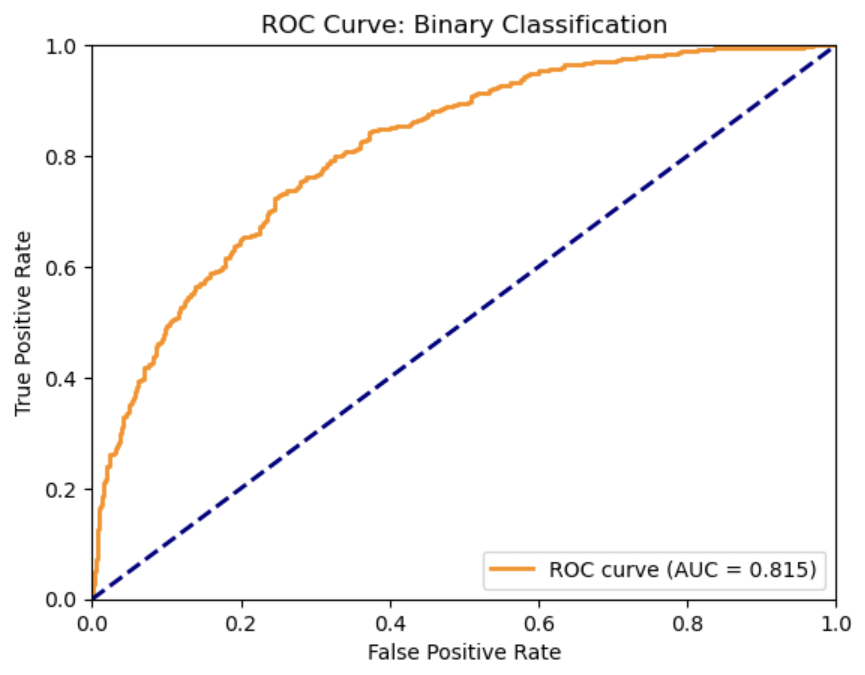
\includegraphics[width=3.6in,height=\textheight]{../images/nn-roc.png}

}

\caption{Neural Network ROC Curve using \texttt{high\_absenteeism}
target}

\end{figure}%

While the binary classification model displayed a solid performance in
predicting absenteeism rates, its ability to identify all high
absenteeism districts is limited. Future improvements could focus on
enhancing recall, possibly by adjusting the decision threshold or
exploring different model architectures, to better detect high
absenteeism districts that require intervention.

The multiclass classification neural network model demonstrated modest
results in classifying school districts into low, medium, and high
absenteeism categories. After training for 18 epochs, the model achieved
a final validation loss of 0.9457. After tuning the model's
hyperparameters, the best-performing configuration utilized three hidden
layers of 256 neurons each, a dropout rate of 0.3, and the RMSprop
optimizer at a learning rate of 0.001.

The model's accuracy, precision, recall, and F1 score can all be derived
from the confusion matrix in Figure 2. In terms of overall performance,
the model's overall accuracy was 0.5523, indicating that 55.23\% of the
model's predictions were correct. While this demonstrates some
predictive capability, it also highlights challenges posed by class
imbalances, where the model may struggle with less dominant absenteeism
categories. The model achieved a precision score of 0.5673, suggesting
that when it predicts a district's absenteeism level, it is correct
56.73\% of the time. This indicates a moderate ability for the model to
avoid false positives. With a recall of 0.5523, the model successfully
identified 55.23\% of the true absenteeism cases across all classes.
This metric highlights the model's limitations in capturing all relevant
instances, particularly with the medium absenteeism bin. Finally, the
model's F1 score of 0.5389 reflects a balance between precision and
recall. This metric suggests that while the model is functional, it
could benefit from adjustments to better address the complexities of the
data.

\begin{figure}[H]

{\centering 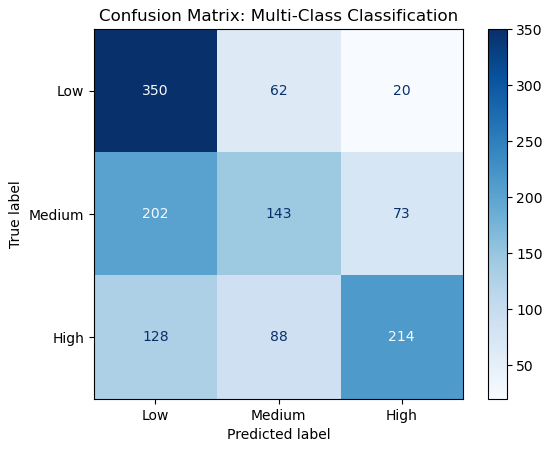
\includegraphics[width=3.6in,height=\textheight]{../images/nn-multi-confusion-matrix.png}

}

\caption{Confusion Matrix for Multi-Class Classification using a Neural
Network}

\end{figure}%

These results highlight the need for enhancements in feature engineering
and possibly exploring alternative model architectures to improve
overall multi-class classification performance.

\subsubsection{Linear Discriminant Analysis \& Quadratic Discriminant
Analysis}\label{linear-discriminant-analysis-quadratic-discriminant-analysis-1}

Two LDA models were trained to predict school districts with
higher-than-average chronic absenteeism. Both predicted a binary
outcome, high\_absenteeism, coded as 1 if a district's chronic
absenteeism rate exceeded 23.6\%---the average rate in the dataset.
Using a standard 80/20 train-test split and 10-fold cross-validation,
the first model was trained on all numerical predictors, yielding an
accuracy of 0.676. Sensitivity was 0.845, while specificity was 0.431.
The second LDA model used a subset of predictors selected through
forward stepwise feature selection aimed at maximizing the Adjusted
R-squared value. This process reduced the number of predictors from 15
to 12. Using the same train-test split and cross-validation approach,
the second model achieved an accuracy of 0.674. However, its sensitivity
decreased slightly to 0.834, while its specificity increased to 0.464.
Based on the confusion matrices of both models, it is evident that while
they are effective at identifying districts with lower chronic
absenteeism, they underperform in accurately predicting districts with
high absenteeism.

The QDA model was trained using all numeric predictors with the intent
to predict the binary high absenteeism variable. The same 80/20
train-test split and 10-fold cross-validation applied to the LDA models
was applied here, yielding an accuracy of 63.8\%. This model has a high
sensitivity of 0.924 while having a very low specificity of 0.237. This
shows that the QDA model performs poorly when predicting high
absenteeism schools, but it does better predict lower absenteeism
schools. Overall, the QDA model performs worse than both LDA models,
suggesting that it overfits the training data. When comparing all the
models, their relative AUC performance when leveraging a ROC plot is
seen in Figure 3.

\begin{figure}[H]

{\centering 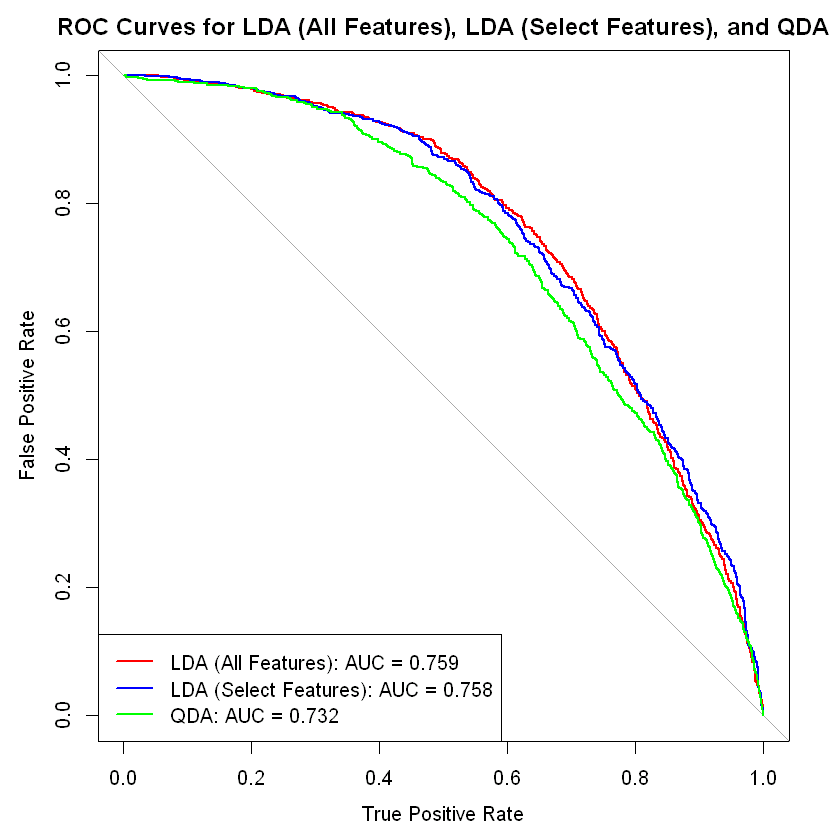
\includegraphics[width=3.6in,height=\textheight]{../images/lda-qda-roc.png}

}

\caption{ROC Curve using \texttt{high\_absenteeism} target}

\end{figure}%

When basing predictions on the Department of Education's average chronic
absenteeism statistic (28\%) the models improved. The first LDA model,
once again using all features as well as the same train-test split and
cross-validation technique, achieved an accuracy of 73.5\%. Its
sensitivity was .918 while its specificity was 0.295. The
feature-selection LDA model achieved an accuracy of 72.9\%. Its
sensitivity and specificity were similar to the first, being 0.919 and
0.269 respectively. Finally, the QDA model resulted in an accuracy of
72.5\%, having a slightly higher specificity at 0.930 and a lower
specificity at 0.229. Figure 4 compares their relative performance based
on AUC.

\begin{figure}[H]

{\centering 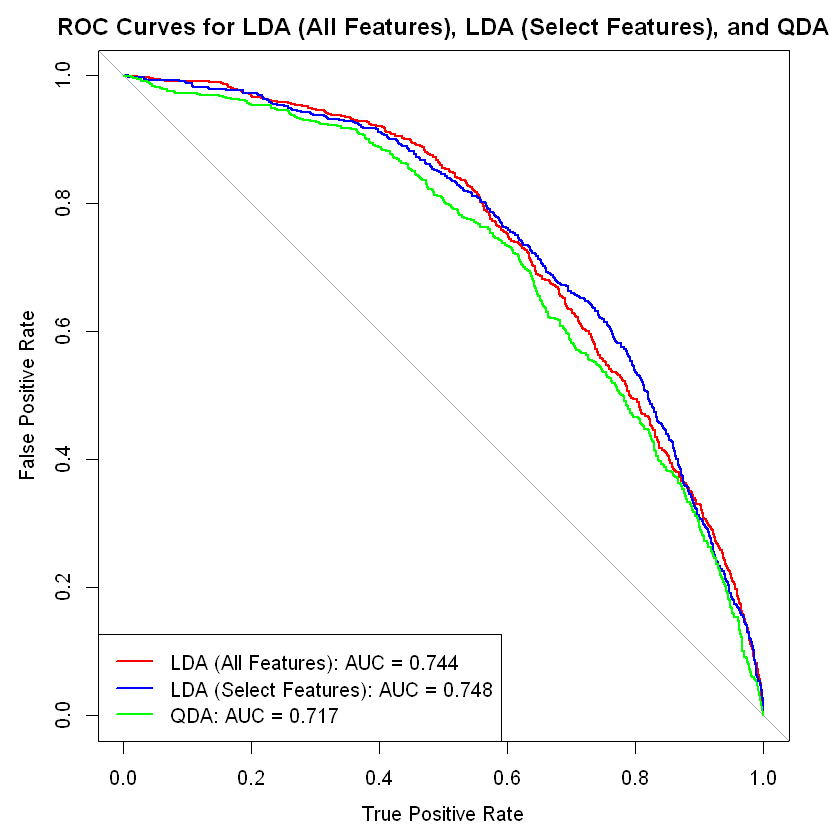
\includegraphics[width=3.6in,height=\textheight]{../images/lda-qda-roc-doe.png}

}

\caption{ROC Curve using \texttt{high\_absenteeism\_doe} target}

\end{figure}%

The remaining models were less successful in predicting the multi-class
classification variable. The first LDA model, which used all numeric
variables with an 80/20 train-test split and 10-fold cross-validation,
achieved an accuracy of 50.9\%. It struggled particularly with
identifying medium-risk school districts while performing better at
predicting low-risk and high-risk districts. The second LDA model, using
the same data split and cross-validation strategy but restricted to 12
numeric predictors selected to maximize the Adjusted R-squared value,
produced similar results. Its accuracy was 49\%, and it also
underperformed in classifying medium-risk districts. Lastly, the QDA
model, trained with the same approach, performed the worst, with an
accuracy of 44\%. The confusion matrix indicated that predictions were
heavily biased toward the low-risk category, resulting in the
misclassification of most medium- and high-risk schools.

\subsubsection{Logistic Regression}\label{logistic-regression-1}

Initially, the team fit logistic regression models to predict high
absenteeism, using both the self-defined and DOE-defined thresholds. In
both cases, the original models showed moderate accuracy but relatively
low sensitivity, particularly when predicting the positive (high
absenteeism) class. To address skewness and potential non-linearity in
key predictors, a log transformation was applied to highly right-skewed
variables, which included all of our feature variables. After
log-transforming these predictors, model performance improved across
both thresholds.

For the self-defined absenteeism threshold, the logistic regression
model's test set accuracy increased from 69.2\% to 71.4\%, and the AUC
improved from 0.72 to 0.76, indicating stronger overall discrimination
between high and low absenteeism districts. Sensitivity increased from
45.7\% to 53.2\%, with only a minor reduction in specificity, suggesting
better identification of schools with high absenteeism without
sacrificing much in the way of correctly identifying low-absenteeism
schools. Similarly, for the DOE-defined threshold, the log-transformed
model achieved a test set accuracy of 77.6\% (compared to 75.4\%
pre-transformation) and an AUC improvement from 0.70 to 0.73.
Sensitivity rose slightly from 29.0\% to 34.5\%, while specificity
remained high at over 90\%, indicating that the model continued to
effectively screen out schools not at high risk while modestly improving
its ability to detect true high-absenteeism cases.

\begin{figure}[H]

{\centering 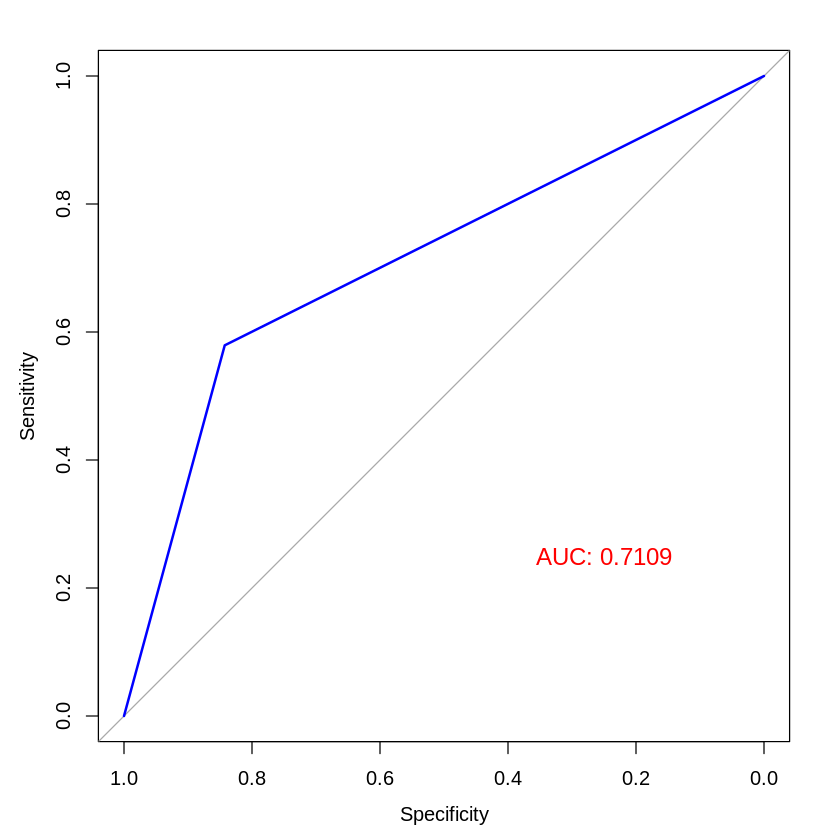
\includegraphics[width=3.6in,height=\textheight]{../images/logistic-roc.png}

}

\caption{ROC Curve using \texttt{high\_absenteeism\_doe} target}

\end{figure}%

In both cases, there was an indication of potential issues with complete
or quasi-complete separation among the predictors for certain
observations. This appeared less extreme after transformation,
suggesting improved model stability. Overall, the log transformation
meaningfully enhanced model calibration and discrimination, particularly
for predictors with heavy-tailed distributions.

\subsubsection{Support Vector Machines}\label{support-vector-machines-1}

Using the self-defined threshold, the SVM model achieved an overall
accuracy of 51\%. The model demonstrated strong recall for identifying
students with high absenteeism (recall = 0.89) but struggled with
detecting low absenteeism cases, where recall was only 0.23. The area
under the ROC curve (AUC) was 0.6591, suggesting moderate discriminative
ability. Despite the relatively high precision for low-absenteeism
students (precision = 0.76), the model's imbalanced sensitivity across
classes indicated a tendency to overpredict high absenteeism. When the
DOE-defined threshold was used, model performance improved. Accuracy
increased to 65\%, and the recall for low-absenteeism students rose to
0.70, while the recall for high-absenteeism students was 0.53. The AUC
similarly improved to 0.6642. These results indicate that the
DOE-defined threshold offered a more balanced classification between the
two groups and provided a slight overall performance gain.

\begin{figure}[H]

{\centering 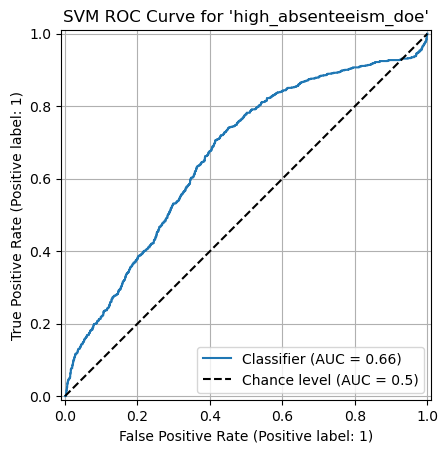
\includegraphics[width=3.6in,height=\textheight]{../images/svm-roc.png}

}

\caption{ROC Curve using \texttt{high\_absenteeism\_doe} target}

\end{figure}%

Alternative kernels were evaluated to investigate model performance
further. When switching to the radial basis function (RBF) kernel, the
model's performance deteriorated substantially. Accuracy dropped to
37\%, and the AUC score fell to 0.4464, indicating performance worse
than random guessing. The model's recall for low-absenteeism students
was particularly poor at just 0.15, suggesting that the RBF kernel was a
poor fit for the data under current tuning parameters. Similarly, the
polynomial kernel produced extremely poor results. The confusion matrix
indicated that the model misclassified nearly all observations,
particularly failing to correctly identify low-absenteeism students.

Finally, hyperparameter tuning on the regularization parameter (C) was
performed to assess potential improvements. A grid search across C
values showed minimal impact on model performance, with accuracy,
recall, and AUC remaining largely unchanged. This suggests that, under
the current feature set and without more extensive feature engineering
or kernel adjustments, the SVM's performance is relatively insensitive
to the level of regularization.

\subsubsection{Random Forests}\label{random-forests-1}

In the binary classification task (predicting whether a district would
exhibit high chronic absenteeism) the Random Forest model achieved an
accuracy of 74\% and an AUC of 0.728. The model performed better on the
majority class (non-high absenteeism), with a precision of 0.76 and
recall of 0.82, while it had slightly lower performance on the high
absenteeism class (precision: 0.72, recall: 0.64). These results
indicate reasonably strong discriminative ability, with a balanced
trade-off between precision and recall.

In the multiclass classification (absenteeism levels as low, medium, or
high) the model achieved an overall accuracy of 58\%. Class-level
performance varied: the model performed best on the low and high
absenteeism classes, with F1-scores of 0.65 and 0.63 respectively, while
performance on the medium category lagged (F1-score: 0.46). This
suggests some difficulty in differentiating medium absenteeism from
adjacent categories. Across both tasks, the student poverty ratio
emerged as the most important feature, highlighting its strong
predictive power for chronic absenteeism risk.

\begin{figure}[H]

{\centering 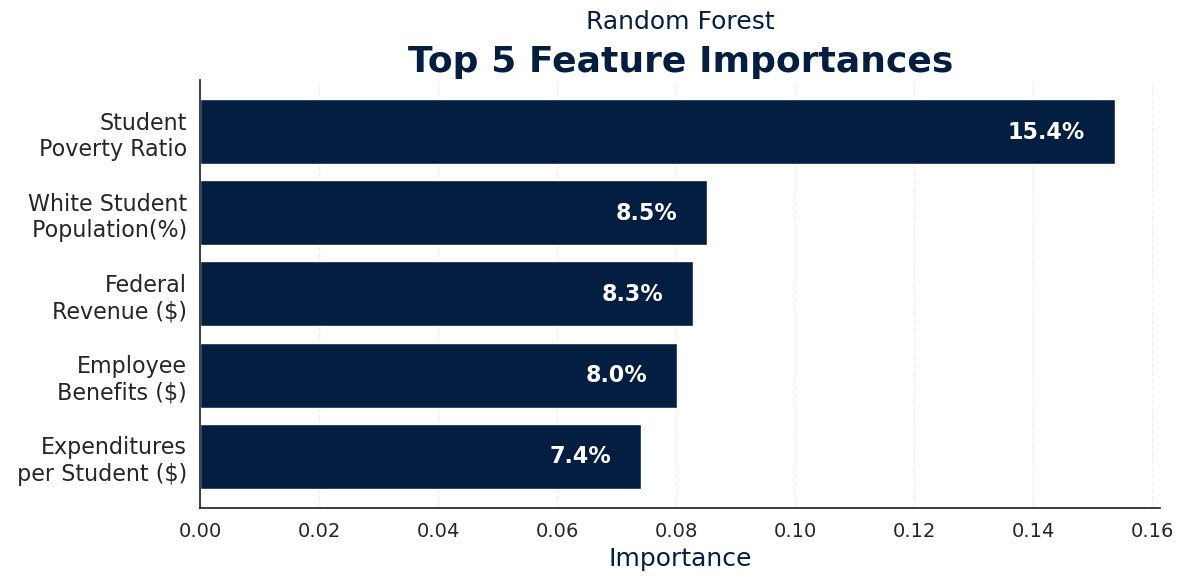
\includegraphics[width=4in,height=\textheight]{../images/feature-importance.png}

}

\caption{Feature Importance Results from Random Forest}

\end{figure}%

\subsubsection{Binary Model Confusion
Matrices}\label{binary-model-confusion-matrices}

The following confusion matrices summarize classification performance
for each of the six binary models predicting high absenteeism. They
highlight each model's ability to correctly identify both high and low
absenteeism districts.

\begin{figure}[H]

{\centering 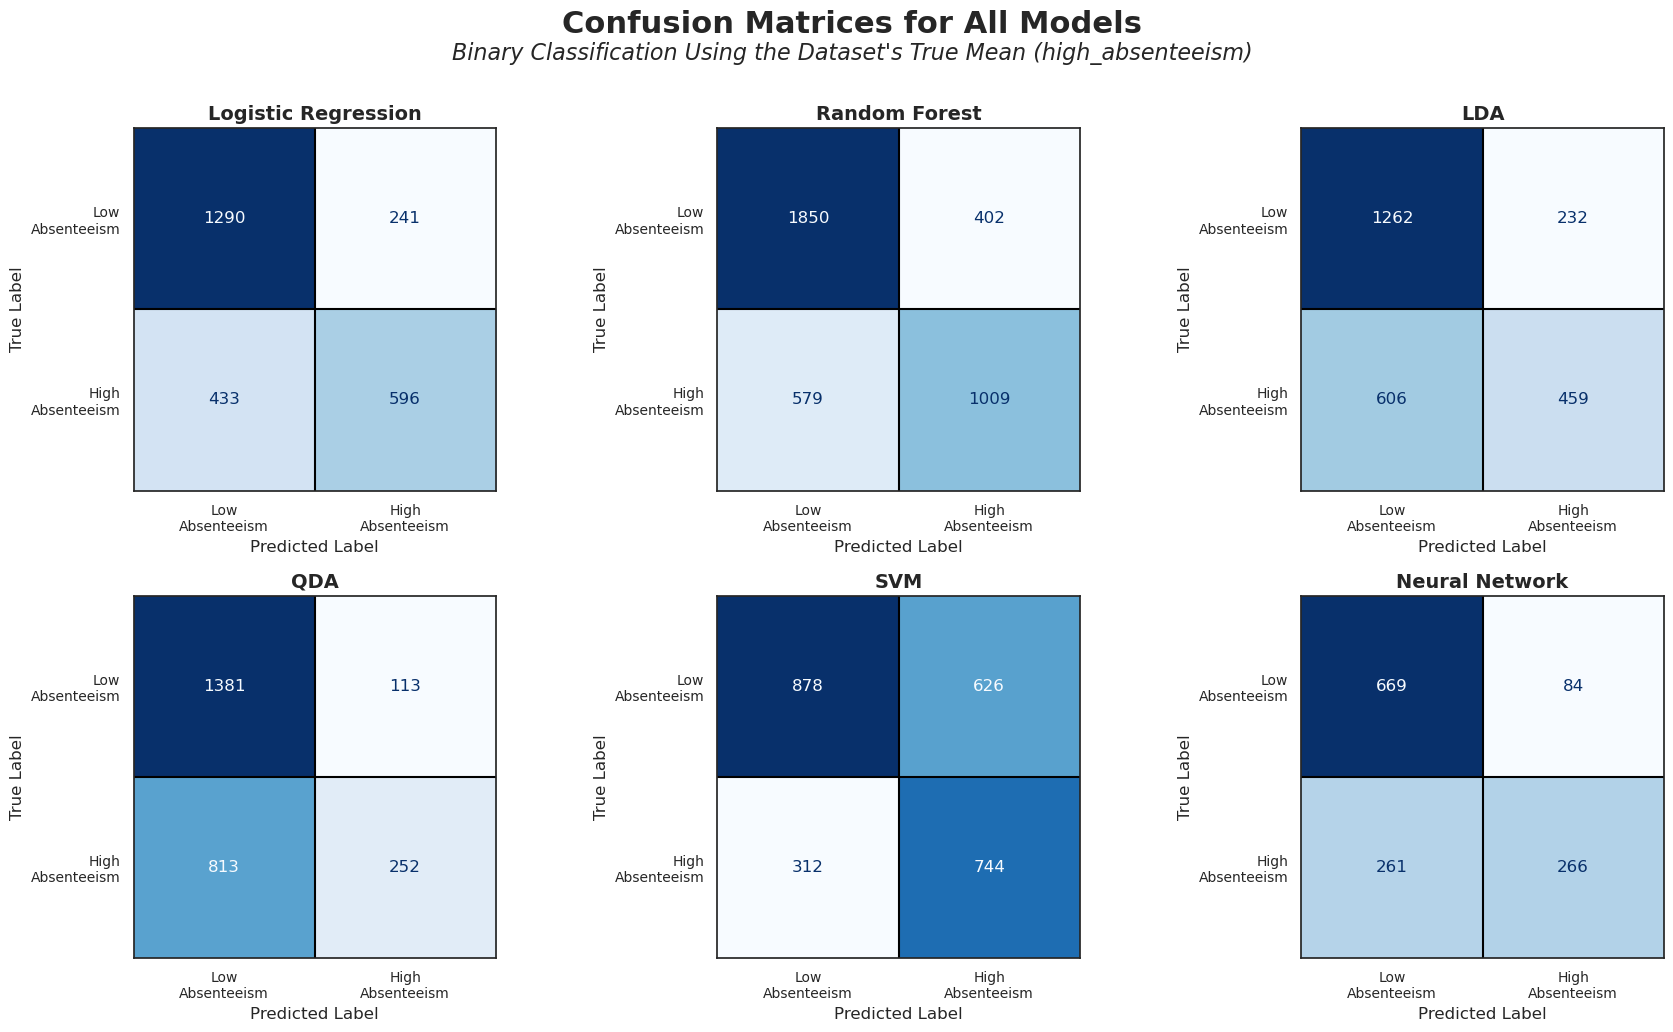
\includegraphics{../images/all-models-conf-mat.png}

}

\caption{Confusion matrices for all binary classification models using
the \texttt{high\_absenteeism} target.}

\end{figure}%

\subsection{Discussion}\label{discussion}

Among the models used in this study, neural networks produced the best
results, outperforming all others in terms of accuracy and balanced
classification metrics. Neural networks excelled at capturing the
complex, nonlinear relationships between district characteristics and
absenteeism outcomes, although at the cost of interpretability.

Random forests also performed well. They offered high predictive
accuracy while maintaining greater interpretability than neural
networks. Through random forests, the team extracted meaningful variable
importance rankings, which provided insight into which district
characteristics most influenced absenteeism rates. Random forests were
particularly helpful in handling feature interactions and
non-linearities without extensive preprocessing. Logistic regression
also performed reasonably well. Despite its simplicity, it provided a
solid baseline and was effective for binary classification. However, it
struggled to capture the complex, nonlinear relationships in the data,
which more flexible models like neural networks and random forests could
better address.

LDA and QDA underperformed significantly compared to the more flexible
models. These methods, while theoretically suited for normally
distributed data, performed poorly due to the violation of their
distributional assumptions in our real-world dataset. This limited their
ability to effectively model the complexities of chronic absenteeism in
school districts. SVMs struggled to achieve high accuracy, especially
when faced with the complexity of our data. Additionally, SVMs lacked
the interpretability provided by models like random forests, which made
understanding their predictions challenging.

A major challenge during this process was dealing with highly correlated
features. Initially, the dataset included detailed information on the
demographic breakdown of chronic absenteeism by subgroups (e.g.,
absenteeism rates by race and disability status). However, many of these
variables were perfectly correlated with the outcome, effectively
leaking the answer into the predictors. Including them would have
resulted in artificially inflated performance without yielding
meaningful insights. As a result, the team removed these features and
focused on broader district-level predictors, such as overall
demographic composition and financial characteristics. This experience
reinforced the importance of careful feature selection to ensure models
are genuinely predictive rather than merely memorizing the outcome.

\subsection{Conclusion}\label{conclusion}

This study provided important insights into the factors that drive
chronic absenteeism across U.S. school districts. Across all models,
especially the variable importance outputs from random forests and
feature weights of logistic regression, the team found that the student
poverty ratio, the percentage of white students, and funding-related
variables (such as state and local revenue per pupil) were consistently
the most important predictors.

Districts with higher poverty rates tended to experience significantly
higher chronic absenteeism, suggesting that broader socioeconomic
disadvantages strongly affect school attendance. Similarly, districts
with higher shares of white students typically had lower absenteeism
rates, though this finding likely reflects deeper structural
inequalities rather than direct causal effects. Less surprisingly,
funding variables played a major role, as districts with greater
financial resources are better positioned to support students and reduce
absenteeism.

Ultimately, the results suggest that efforts to address chronic
absenteeism should focus not just on in-school policies but also on
broader socioeconomic conditions and resource allocation. By identifying
poverty and underfunding as key risk factors, our models highlight areas
where interventions could be most impactful.

\subsection{References}\label{references}

\phantomsection\label{refs}
\begin{CSLReferences}{1}{0}
\bibitem[\citeproctext]{ref-bowen2022revealing}
Bowen, Francis, Carolyn Gentle-Genitty, Janaina Siegler, and Marlin
Jackson. 2022. {``Revealing Underlying Factors of Absenteeism: A Machine
Learning Approach.''} \emph{Frontiers in Psychology} 13: 958748.

\bibitem[\citeproctext]{ref-egorov2025chronic}
Egorov, Danyela Souza. 2025. {``Chronic Absenteeism Is Hampering School
Improvement Efforts in New York City.''}
\url{https://manhattan.institute/article/chronic-absenteeism-hampering-school-improvement-efforts-new-york-city}.

\bibitem[\citeproctext]{ref-jarbou2022deep}
Jarbou, Mohammed, Daehan Won, Jennifer Gillis-Mattson, and Raymond
Romanczyk. 2022. {``Deep Learning-Based School Attendance Prediction for
Autistic Students.''} \emph{Scientific Reports} 12 (1): 1431.

\bibitem[\citeproctext]{ref-used2024chronic}
U.S. Department of Education. 2024a. {``Chronic Absenteeism.''}
\url{https://www.ed.gov/teaching-and-administration/supporting-students/chronic-absenteeism}.

\bibitem[\citeproctext]{ref-ede2021chronic}
---------. 2024b. {``Chronic Absenteeism Dashboard: 2021--2022.''}
\url{https://eddataexpress.ed.gov/dashboard/chronic-absenteeism/2021-2022}.

\bibitem[\citeproctext]{ref-wu2024leveraging}
Wu, Tiffany, and Christina Weiland. 2024. {``Leveraging Modern Machine
Learning to Improve Early Warning Systems and Reduce Chronic Absenteeism
in Early Childhood. EdWorkingPaper No. 24-1081.''} \emph{Annenberg
Institute for School Reform at Brown University}.

\end{CSLReferences}

\newpage

\subsection{Appendix}\label{appendix}

\begin{figure}[H]

{\centering 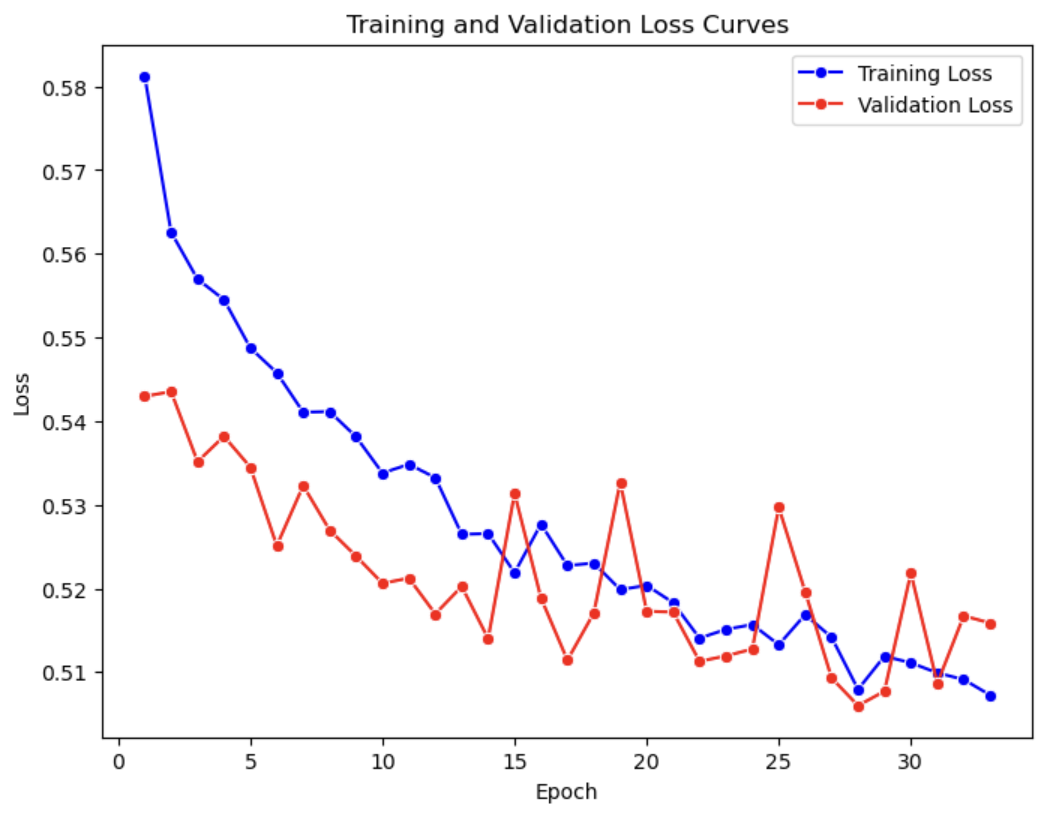
\includegraphics[width=3.6in,height=\textheight]{../images/nn-binary-loss-curves.png}

}

\caption{Neural Network Binary Classification Loss Curves}

\end{figure}%%
\begin{figure}[H]

{\centering 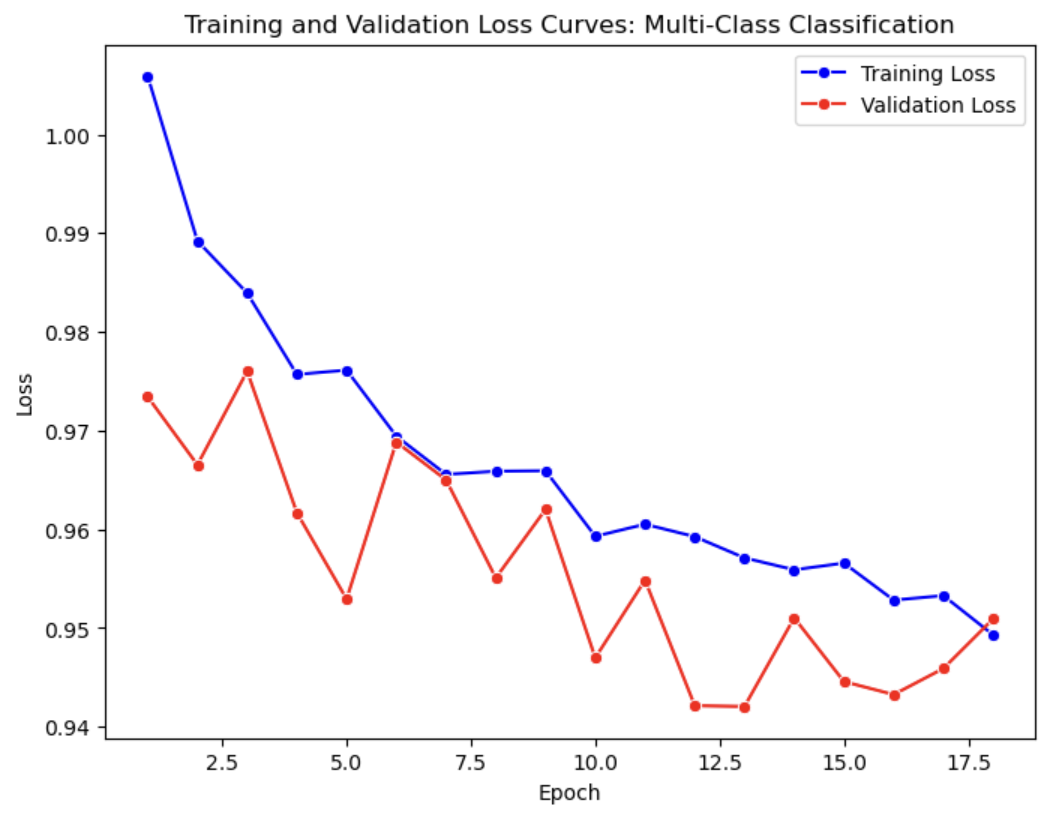
\includegraphics[width=3.6in,height=\textheight]{../images/nn-multi-loss-curves.png}

}

\caption{Neural Network Multi-Class Classification Loss Curves}

\end{figure}%%
\begin{figure}[H]

{\centering 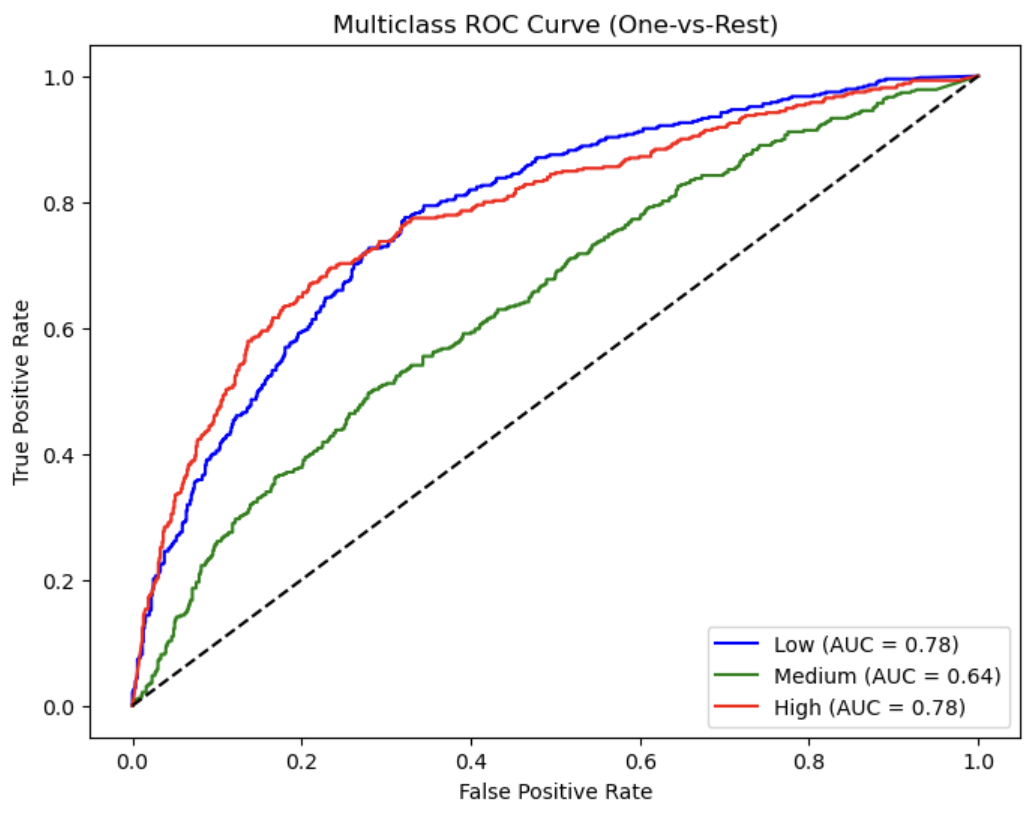
\includegraphics[width=3.6in,height=\textheight]{../images/nn-multi-roc.png}

}

\caption{Neural Network Multi-Class Classification ROC Curve}

\end{figure}%%
\begin{figure}[H]

{\centering 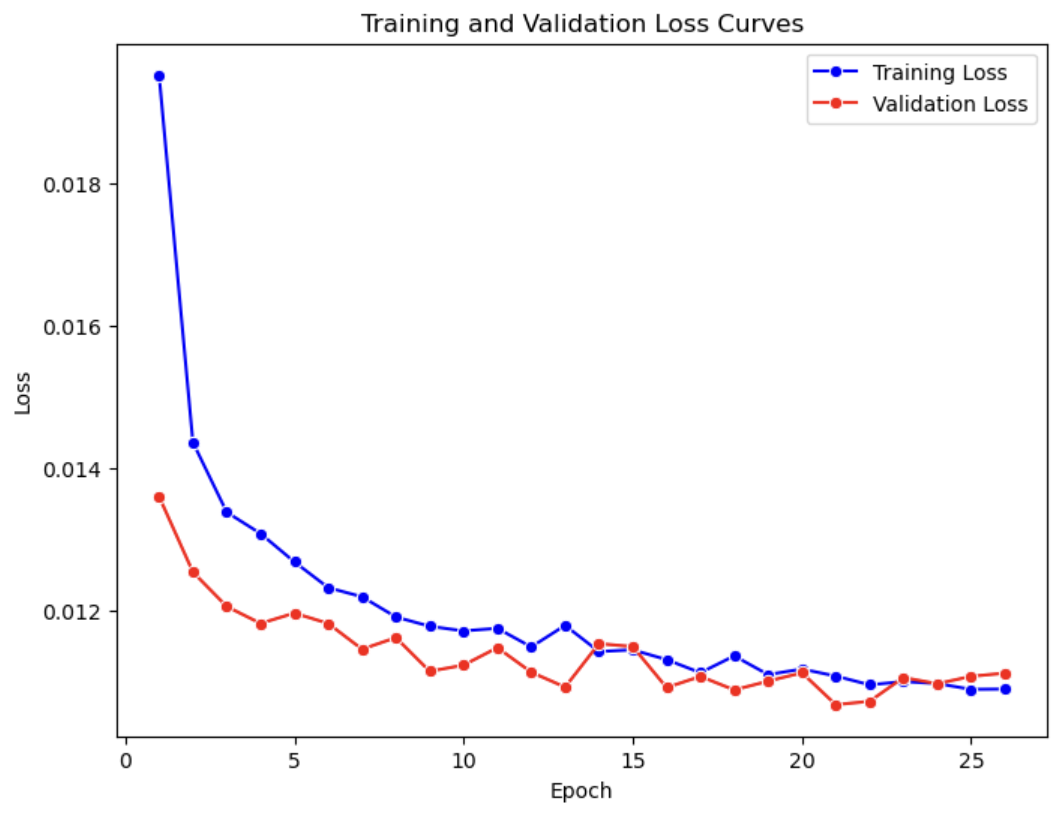
\includegraphics[width=3.6in,height=\textheight]{../images/nn-regression-loss-curves.png}

}

\caption{Neural Network Regression Loss Curves}

\end{figure}%%
\begin{figure}[H]

{\centering 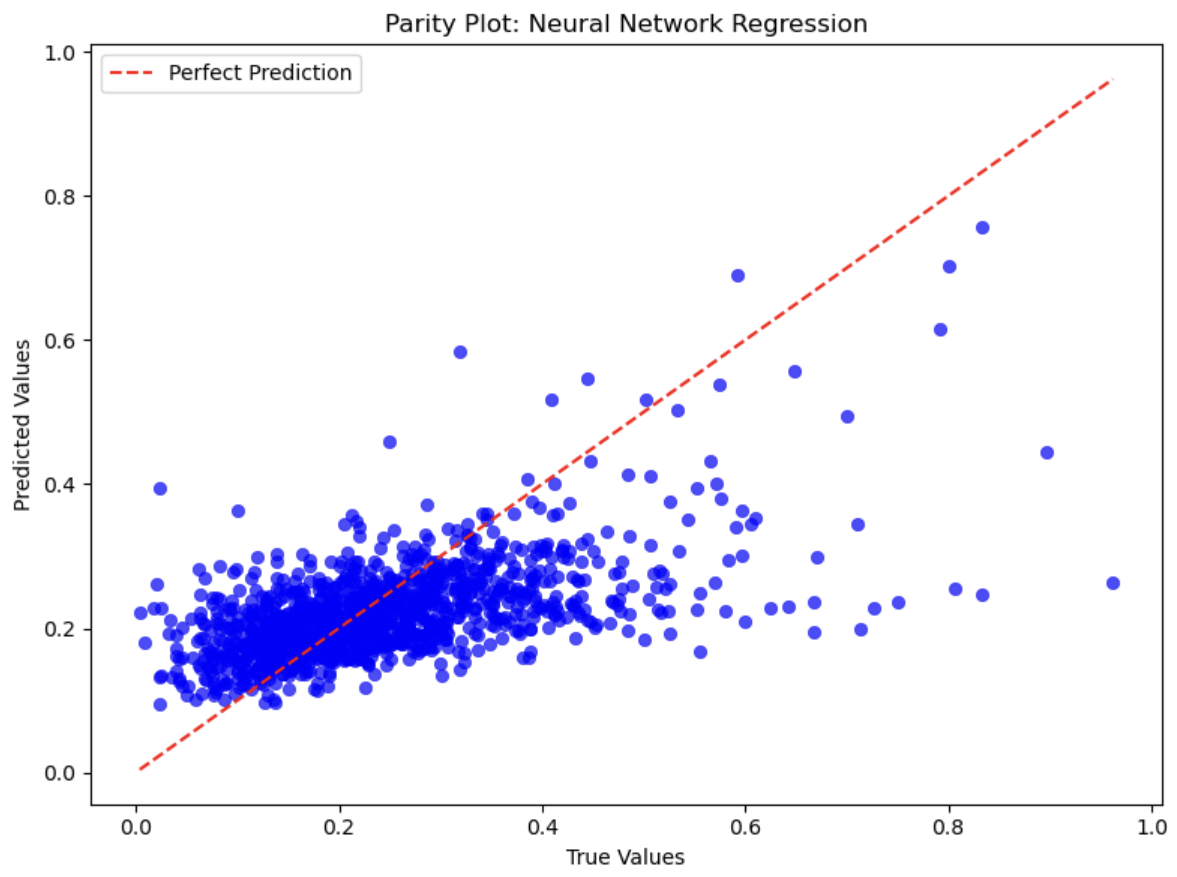
\includegraphics[width=3.6in,height=\textheight]{../images/nn-regression-parity-plot.png}

}

\caption{Neural Network Regression Parity Plot}

\end{figure}%




\end{document}
